\chapter{DESENVOLVIMENTO}

Texto do capítulo. Os dados completos estão na Tabela \ref{tab:survey}, no Apêndice B.

\section{Quadro longo com cabeçalho repetido}

Quadro que continua em outra página, apresentado no Quadro~\ref{frame:long}.

{\small
\begin{longtable}{|p{1.8cm}|p{3.2cm}|p{7.0cm}|p{2.1cm}|}
\caption{Título do quadro longo} \label{frame:long} \\
\hline
\textbf{Código} & \textbf{Nome} & \textbf{Descrição} & \textbf{Prioridade} \\ \hline
\endfirsthead
\hline
\textbf{Código} & \textbf{Nome} & \textbf{Descrição} & \textbf{Prioridade} \\ \hline
\endhead
\hline
\continuedrow{4} \\
\endfoot
\hline
\sourcerow{4} \\
\endlastfoot
{[RF001]} & Nome & Descrição. & Obrigatório \\ \hline
{[RF002]} & Nome & Descrição. & Desejável \\ \hline
\end{longtable}
}

\section{Quadro de atributo e valor}

Quadro com rótulos na primeira coluna, apresentado no Quadro~\ref{frame:key_value}.

{\small
\begin{longtable}{|l|p{10cm}|}
\caption{Título do quadro de atributo e valor}
\label{frame:key_value} \\
\hline
\endfirsthead
\hline
\endhead
\hline
\continuedrow{2} \\
\endfoot
\hline
\sourcerow{2} \\
\endlastfoot
\textbf{Atributo} & Valor. \\ \hline
\textbf{Atributo} & Valor. \\ \hline
\end{longtable}
}

\section{Caso de uso}

Descrição de caso de uso, apresentada no Quadro~\ref{frame:uc001}.

{\small
\begin{longtable}{|p{3.5cm}|p{11.0cm}|}
\caption{[UC001] Nome do caso de uso} \label{frame:uc001} \\
\endfirsthead
\continuedrow{2} \\
\endfoot
\hline
\sourcerow{2} \\
\endlastfoot
\hline
\textbf{Caso de uso} & [UC001] Nome do caso de uso \\ \hline
\textbf{Ator(es)} & Ator \\ \hline
\textbf{Motivação} & Motivação do caso de uso. \\ \hline
\textbf{Fluxo Principal} &
1. Passo;\newline
2. Passo;\newline
3. Passo.
\\ \hline
\textbf{Fluxo Alternativo} &
a. Condição alternativa:\newline
\hspace*{1em}i. Passo;\newline
\hspace*{1em}ii. Passo.
\\ \hline
\end{longtable}
}

\section{Quadro com lista na célula}

Quadro com itens dentro da célula, apresentado no Quadro~\ref{frame:list_cell}.

{\small
\begin{longtable}{|p{4cm}|p{10.5cm}|}
\caption{Título do quadro com lista} \label{frame:list_cell} \\
\hline
\textbf{Coluna 1} & \textbf{Coluna 2} \\ \hline
\endfirsthead
\hline
\textbf{Coluna 1} & \textbf{Coluna 2} \\ \hline
\endhead
\hline
\continuedrow{2} \\
\endfoot
\hline
\sourcerow{2} \\
\endlastfoot

Item &
\begin{minipage}[t]{\linewidth}
\begin{itemize}[noitemsep,topsep=2pt,leftmargin=*]
    \item Conteúdo.
    \item Conteúdo.
\end{itemize}
\end{minipage} \\ \hline

\end{longtable}
}

\section{Figuras lado a lado}

Figuras lado a lado, apresentadas nas Figuras~\ref{fig:side_1} e \ref{fig:side_2}.

\noindent
\begin{minipage}[t]{0.42\textwidth}
    \centering
    \captionof{figure}{Título da figura.}
    \label{fig:side_1}
    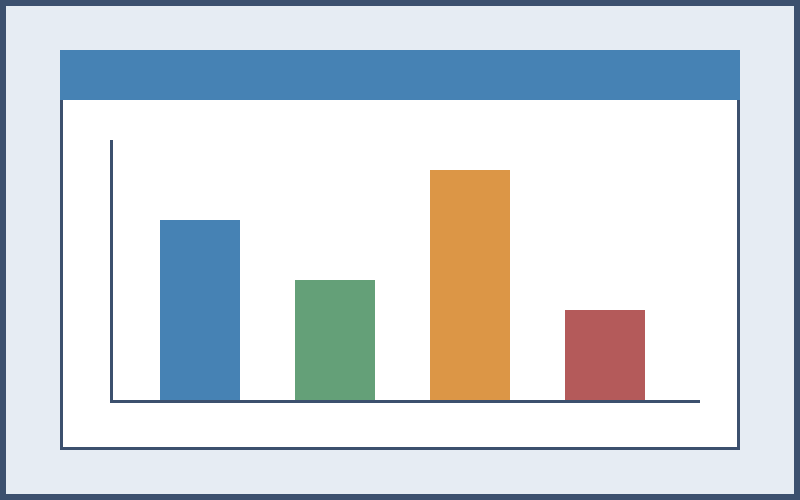
\includegraphics[width=\textwidth]{images/example.png}
    \authorssource
\end{minipage}
\hfill
\begin{minipage}[t]{0.42\textwidth}
    \centering
    \captionof{figure}{Título da figura.}
    \label{fig:side_2}
    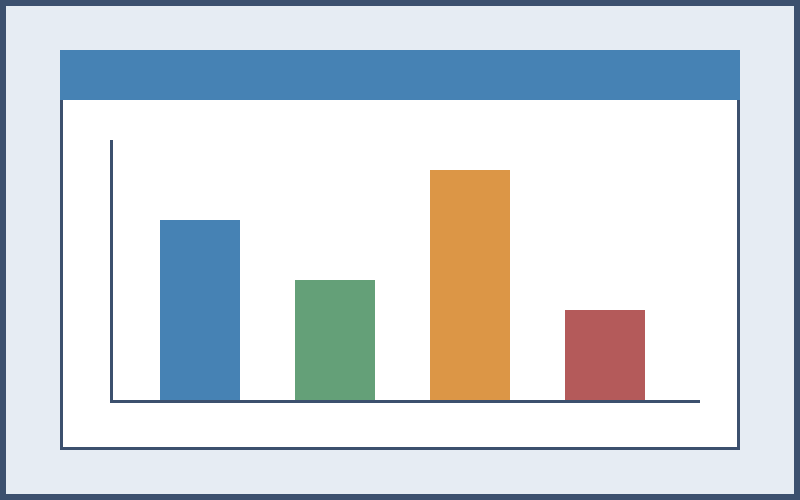
\includegraphics[width=\textwidth]{images/example.png}
    \authorssource
\end{minipage}

\vspace{16pt}
